\section{Preventivo di periodo}
Per facilitare la lettura delle tabelle vengono utilizzate le seguenti sigle per identificare i diversi ruoli e per ognuno di essi vengono indicati i relativi costi/h: \begin{itemize}
\item \textbf{Re}: \textit{Responsabile} 30€/h;
\item \textbf{Am}: \textit{Amministratore} 20€/h;
\item \textbf{An}: \textit{Analista} 25€/h;
\item \textbf{Pt}: \textit{Progettista} 22€/h;
\item \textbf{Pm}: \textit{Programmatore} 15€/h;
\item \textbf{Ve}: \textit{Verificatore} 15€/h.
\end{itemize}
Inoltre, se le ore ricoperte in un determinato ruolo fossero nulle, la cella presenterà il simbolo "-" per indicarne l'assenza.
 
\subsection{Fase di Analisi}
\subsubsection{Distribuzione oraria}
In questa fase, i ruoli sono così suddivisi:
\begin{table}[H]
\centering\renewcommand{\arraystretch}{1.5}
\caption{Distribuzione delle ore nella fase di Analisi}
\vspace{0.2cm}
\begin{tabular}{ c c c c c c c c }
\rowcolor{redafk}
\textcolor{white}{\textbf{Nominativo}} & \textcolor{white}{\textbf{Re}} &
\textcolor{white}{\textbf{Am}} & \textcolor{white}{\textbf{An}} &
\textcolor{white}{\textbf{Pt}} & \textcolor{white}{\textbf{Pm}} &
\textcolor{white}{\textbf{Ve}} & \textcolor{white}{\textbf{Totale}} \\
Simone Federico Bergamin & 6 & 7 & 20 & - & - & 9 & 42 \\
Alessandro Canesso & 8 & 6 & 16 & - & - & 12 & 42 \\
Victor Dutca & 9 & - & 15 & - & - & 16 & 40 \\
Fouad Farid & 7 & 7 & 12 & 6 & - & 8 & 40 \\
Simone Meneghin & - & 8 & 14 & 10 & - & 10 & 42 \\
Olivier Utshudi & - & 8 & 13 & 8 & - & 13 & 42 \\
Davide Zilio & 4 & 5 & 17 & - & - & 14 & 40 \\
\rowcolor{lastrowcolor}
\textbf{Ore totali ruolo} & \textbf{34} & \textbf{41} & \textbf{107} & \textbf{24} & \textbf{0} & \textbf{82} & \textbf{288} \\
\end{tabular}
\end{table}
 
\pagebreak
 
I dati ottenuti sono riassunti nel seguente istogramma:
\begin{figure}[H]
\centering
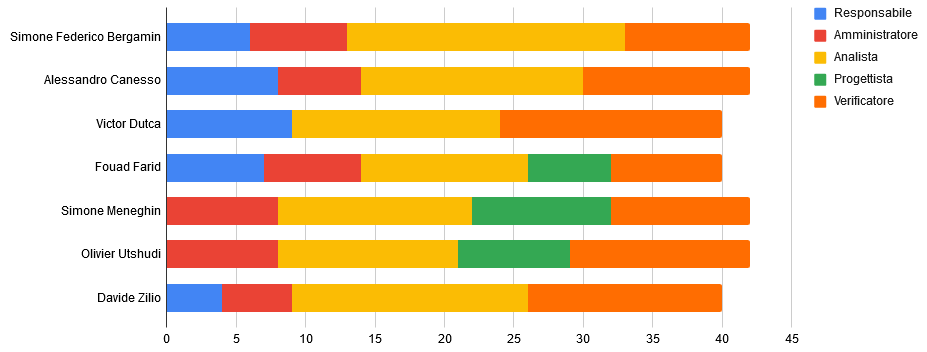
\includegraphics[scale=0.60]{img/grafici/tabella_fase_analisi.png}
\caption{Istogramma della ripartizione delle ore per ruolo nella fase di Analisi}
\end{figure}
 
\subsubsection{Prospetto economico}
In questa fase il costo per ogni ruolo è il seguente:
 
%tabella costi
\begin{table}[H]
\centering\renewcommand{\arraystretch}{1.5}
\caption{Prospetto dei costi nella fase di Analisi}
\vspace{0.2cm}
\begin{tabular}{ c c c  }
\rowcolor{redafk}
\textcolor{white}{\textbf{Ruolo}} & \textcolor{white}{\textbf{Ore}} &
\textcolor{white}{\textbf{Costo}}  \\
Responsabile & 34 & 1020€ \\
Amministratore & 41 & 820€ \\
Analista & 107 & 2675€ \\
Progettista & 24 & 528€ \\
Programmatore & 0 & 0€  \\
Verificatore & 82 & 1230€  \\
\rowcolor{lastrowcolor}
\textbf{Totale} & \textbf{288} & \textbf{6273€}  \\
\end{tabular}
\end{table}
 
I dati ottenuti sono riassunti nel seguente areogramma:
\begin{figure}[H]
\centering
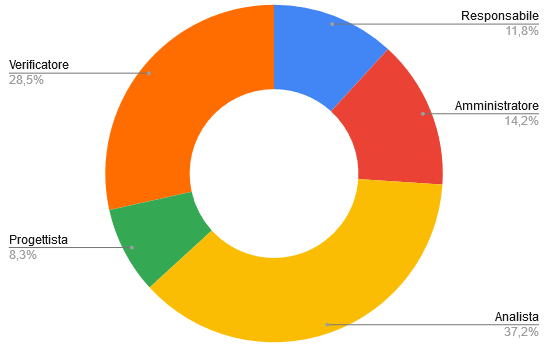
\includegraphics[scale=0.60]{img/grafici/torta_fase_analisi_prospetto_economico.png}
\caption{Areogramma della ripartizione dei costi per ruolo nella fase di Analisi}
\end{figure}
 
%--------------------------------------------------
 
\subsection{Fase di Progettazione e codifica per la Tecnology Baseline}
\subsubsection{Distribuzione oraria}
In questa fase i ruoli sono così suddivisi:
\begin{table}[H]
\centering\renewcommand{\arraystretch}{1.5}
\caption{Distribuzione delle ore nella fase di Progettazione e codifica per la Technology Baseline}
\vspace{0.2cm}
\begin{tabular}{ c c c c c c c c }
\rowcolor{redafk}
\textcolor{white}{\textbf{Nominativo}} & \textcolor{white}{\textbf{Re}} &
\textcolor{white}{\textbf{Am}} & \textcolor{white}{\textbf{An}} &
\textcolor{white}{\textbf{Pt}} & \textcolor{white}{\textbf{Pm}} &
\textcolor{white}{\textbf{Ve}} & \textcolor{white}{\textbf{Totale}} \\
Simone Federico Bergamin & - & - & 10 & 7 & 5 & 8 & 30 \\
Alessandro Canesso & - & 5 & - & 10 & 9 & 8 & 32 \\
Victor Dutca & 3 & 6 & 4 & 10 & 7 & - & 30 \\
Fouad Farid & - & 5 & - & 14 & - & 11 & 30 \\
Simone Meneghin & 6 & - & 8 & 10 & 6 & - & 30 \\
Olivier Utshudi & - & 4 & - & 8 & 6 & 12 & 30 \\
Davide Zilio & 3 & - & 13 & - & - & 14 & 30 \\
\rowcolor{lastrowcolor}
\textbf{Ore totali ruolo} & \textbf{12} & \textbf{20} & \textbf{35} & \textbf{59} & \textbf{33} & \textbf{53} & \textbf{212} \\
\end{tabular}
\end{table}
 
I dati ottenuti sono riassunti nel seguente istogramma:
\begin{figure}[H]
\centering
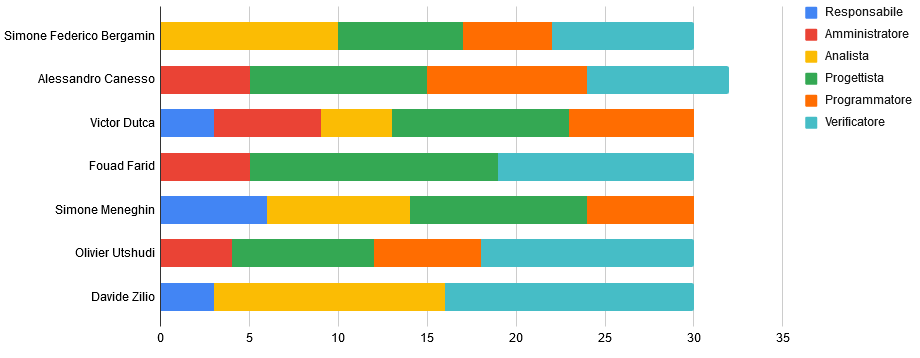
\includegraphics[scale=0.60]{img/grafici/tabella_fase_prog_architetturale.png}
\caption{Istogramma della ripartizione delle ore per ruolo nella fase di Progettazione e codifica per la Technology Baseline}
\end{figure}
 
\subsubsection{Prospetto economico}
In questa fase il costo per ogni ruolo è il seguente:
 
%tabella costi
\begin{table}[H]
\centering\renewcommand{\arraystretch}{1.5}
\caption{Prospetto dei costi nella fase di Progettazione e codifica per la Technology Baseline}
\vspace{0.2cm}
\begin{tabular}{ c c c }
\rowcolor{redafk}
\textcolor{white}{\textbf{Ruolo}} & \textcolor{white}{\textbf{Ore}} &
\textcolor{white}{\textbf{Costo}}  \\
Responsabile & 12 & 360€ \\
Amministratore & 20 & 400€ \\
Analista & 35 & 875€ \\
Progettista & 59 & 1298€ \\
Programmatore & 33 & 495€  \\
Verificatore & 53 & 795€  \\
\rowcolor{lastrowcolor}
\textbf{Totale} & \textbf{212} & \textbf{4223€}  \\
\end{tabular}
\end{table}
 
I dati ottenuti sono riassunti nel seguente areogramma:
\begin{figure}[H]
\centering
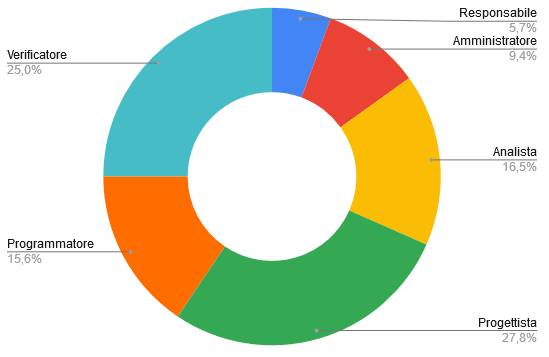
\includegraphics[scale=0.60]{img/grafici/torta_fase_prog_architetturale.png}
\caption{Areogramma della ripartizione dei costi per ruolo nella fase di Progettazione e codifica per la Technology Baseline}
\end{figure}
 
%--------------------------------------------------
 
\subsection{Fase di Progettazione di dettaglio e codifica}
\subsubsection{Distribuzione oraria}
In questa fase i ruoli sono così suddivisi:
\begin{table}[H]
\centering\renewcommand{\arraystretch}{1.5}
\caption{Distribuzione delle ore nella fase di Progettazione di dettaglio e codifica}
\vspace{0.2cm}
\begin{tabular}{ c c c c c c c c }
\rowcolor{redafk}
\textcolor{white}{\textbf{Nominativo}} & \textcolor{white}{\textbf{Re}} &
\textcolor{white}{\textbf{Am}} & \textcolor{white}{\textbf{An}} &
\textcolor{white}{\textbf{Pt}} & \textcolor{white}{\textbf{Pm}} &
\textcolor{white}{\textbf{Ve}} & \textcolor{white}{\textbf{Totale}} \\
Simone Federico Bergamin & - & 6 & - & 12 & 18 & 12 & 48 \\
Alessandro Canesso & 4 & 3 & - & 10 & 18 & 11 & 46 \\
Victor Dutca & - & 8 & - & 10 & 20 & 10 & 48 \\
Fouad Farid & 4 & - & - & 12 & 20 & 12 & 48 \\
Simone Meneghin & 2 & - & - & 12 & 22 & 14 & 50 \\
Olivier Utshudi & 8 & - & - & 8 & 22 & 12 & 50 \\
Davide Zilio & - & 6 & - & 10 & 20 & 12 & 48 \\
\rowcolor{lastrowcolor}
\textbf{Ore totali ruolo} & \textbf{18} & \textbf{23} & \textbf{0} & \textbf{74} & \textbf{140} & \textbf{83} & \textbf{338} \\
\end{tabular}
\end{table}
 
I dati ottenuti sono riassunti nel seguente istogramma:
\begin{figure}[H]
\centering
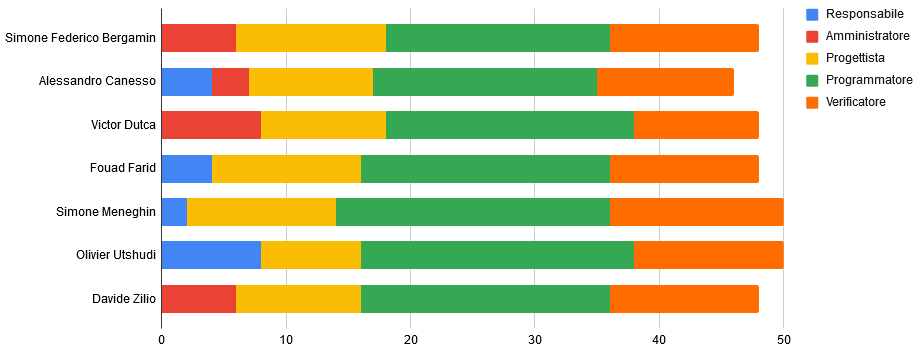
\includegraphics[scale=0.60]{img/grafici/tabella_fase_prog_cod.png}
\caption{Istogramma della ripartizione delle ore per ruolo nella fase di Progettazione di dettaglio e codifica}
\end{figure}
 
\subsubsection{Prospetto economico}
In questa fase il costo per ogni ruolo è il seguente:
 
%tabella costi
\begin{table}[H]
\centering\renewcommand{\arraystretch}{1.5}
\caption{Prospetto dei costi nella fase di Progettazione di dettaglio e codifica}
\vspace{0.2cm}
\begin{tabular}{ c c c }
\rowcolor{redafk}
\textcolor{white}{\textbf{Ruolo}} & \textcolor{white}{\textbf{Ore}} &
\textcolor{white}{\textbf{Costo}}  \\
Responsabile & 18 & 540€ \\
Amministratore & 23 & 460€ \\
Analista & 0 & 0€ \\
Progettista & 74 & 1628€ \\
Programmatore & 140 & 2100€  \\
Verificatore & 83 & 1245€  \\
\rowcolor{lastrowcolor}
\textbf{Totale} & \textbf{338} & \textbf{5973€}  \\
\end{tabular}
\end{table}
 
I dati ottenuti sono riassunti nel seguente areogramma:
\begin{figure}[H]
\centering
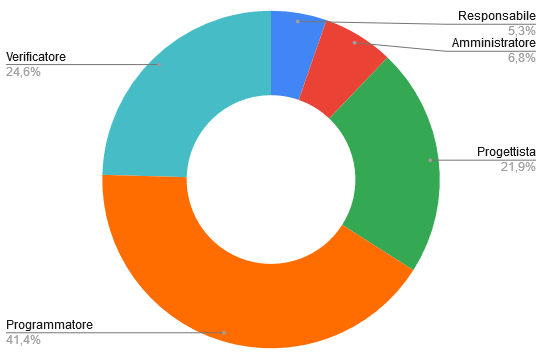
\includegraphics[scale=0.60]{img/grafici/torta_fase_prog_cod.png}
\caption{Areogramma della ripartizione dei costi per ruolo nella fase di Progettazione di dettaglio e codifica}
\end{figure}

%------------------------------------

\subsection{Fase di Validazione e collaudo}
\subsubsection{Distribuzione oraria}
In questa fase i ruoli sono così suddivisi:

%tabella ore
\begin{table}[H]
\centering\renewcommand{\arraystretch}{1.5}
\caption{Validazione e Collaudo}
\vspace{0.2cm}
\begin{tabular}{ c c c c c c c c }
\rowcolor{redafk}
\textcolor{white}{\textbf{Nominativo}} & \textcolor{white}{\textbf{Re}} & 
\textcolor{white}{\textbf{Am}} & \textcolor{white}{\textbf{An}} &
\textcolor{white}{\textbf{Pt}} & \textcolor{white}{\textbf{Pm}} &
\textcolor{white}{\textbf{Ve}} & \textcolor{white}{\textbf{Totale}} \\
Simone Federico Bergamin 	& 5 	& - 	& - 	& - 	& 8 	& 12 	& 25 \\
Alessandro Canesso 			& 4 	& 4 	& - 	& - 	& - 	& 15 	& 23 \\
Victor Dutca 				& 5 	& - 	& - 	& - 	& 5 	& 15 	& 25 \\
Fouad Farid					& - 	& 6 	& - 	& - 	& 7 	& 12 	& 25 \\
Simone Meneghin 			& - 	& 9 	& - 	& - 	& - 	& 16 	& 25 \\
Olivier Utshudi 			& - 	& 4 	& - 	& 4 	& 5 	& 12 	& 25 \\
Davide Zilio 				& 6 	& - 	& - 	& 8 	& - 	& 11 	& 25 \\
\rowcolor{lastrowcolor}
\textbf{Ore totali ruolo} & \textbf{20} & \textbf{23} & \textbf{0} & \textbf{12} & \textbf{25} & \textbf{93} & \textbf{173} \\
\end{tabular}
\end{table}

I dati ottenuti sono riassunti nel seguente istogramma: 
\begin{figure}[H]
\centering
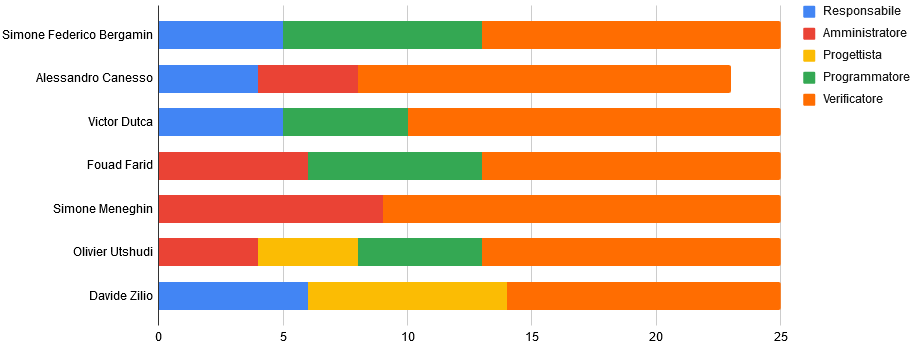
\includegraphics[scale=0.60]{img/grafici/tabella_fase_val_col.png}
\caption{Istogramma della ripartizione delle ore per ruolo nella fase di Validazione e collaudo}
\end{figure}

\subsubsection{Prospetto economico}
In questa fase il costo per ogni ruolo è il seguente:

%tabella costi
\begin{table}[H]
\centering\renewcommand{\arraystretch}{1.5}
\caption{Prospetto dei costi nella fase di Validazione e collaudo}
\vspace{0.2cm}
\begin{tabular}{ c c c }
\rowcolor{redafk}
\textcolor{white}{\textbf{Ruolo}} & \textcolor{white}{\textbf{Ore}} & 
\textcolor{white}{\textbf{Costo}}  \\
Responsabile & 20 & 600€ \\
Amministratore & 23 & 460€ \\
Analista & - & - \\
Progettista	& 12 & 264€ \\
Programmatore & 25 & 375€  \\
Verificatore & 93 & 1395€  \\
\rowcolor{lastrowcolor}
\textbf{Totale} & \textbf{173} & \textbf{3094€}  \\
\end{tabular}
\end{table}

I dati ottenuti si possono riassumere nel seguente areogramma:
\begin{figure}[H]
\centering
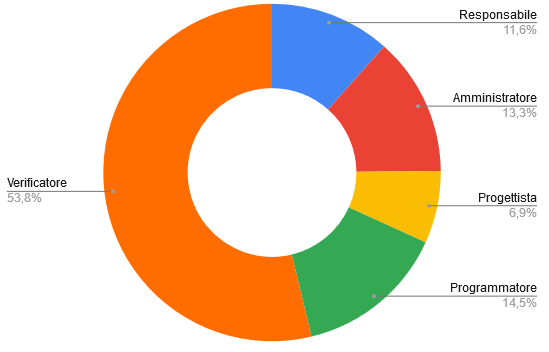
\includegraphics[scale=0.60]{img/grafici/torta_fase_val_col.png}
\caption{Areogramma della ripartizione dei costi per ruolo nella fase di Validazione e collaudo}
\end{figure}


\subsection{Riepilogo}
\subsubsection{Ore rendicontate con investimento}
\paragraph{Distribuzione oraria} \mbox{} \\ \mbox{} \\
Vengono riportate il totale delle ore del progetto in cui sono presenti le ore di investimento e le
ore rendicontate a carico del committente:

%tabella ore
\begin{table}[H]
\centering\renewcommand{\arraystretch}{1.5}
\caption{Distribuzione totale delle ore dell'intero progetto con investimento}
\vspace{0.2cm}
\begin{tabular}{ c c c c c c c c }
\rowcolor{redafk}
\textcolor{white}{\textbf{Nominativo}} & \textcolor{white}{\textbf{Re}} & 
\textcolor{white}{\textbf{Am}} & \textcolor{white}{\textbf{An}} &
\textcolor{white}{\textbf{Pt}} & \textcolor{white}{\textbf{Pm}} &
\textcolor{white}{\textbf{Ve}} & \textcolor{white}{\textbf{Totale}} \\
Simone Federico Bergamin 	& 11 	& 13 	& 30 	& 19 	& 31 	& 41 	& 145 \\
Alessandro Canesso 			& 16 	& 18 	& 16 	& 20 	& 27 	& 46 	& 143 \\
Victor Dutca 				& 17	& 14 	& 19 	& 20 	& 32 	& 41 	& 143 \\
Fouad Farid					& 11	& 18 	& 12 	& 32 	& 27 	& 43 	& 143 \\
Simone Meneghin 			& 8 	& 17 	& 22 	& 32 	& 28 	& 40 	& 147 \\
Olivier Utshudi 			& 8 	& 16 	& 13 	& 28 	& 33 	& 49 	& 147 \\
Davide Zilio 				& 13 	& 11 	& 30 	& 18 	& 20 	& 51 	& 143 \\
\rowcolor{lastrowcolor}
\textbf{Ore totali ruolo} & \textbf{84} & \textbf{107} & \textbf{142} & \textbf{169} & \textbf{198} & \textbf{311} & \textbf{1011} \\
\end{tabular}
\end{table}

Una rappresentazione visiva della suddivisione oraria viene data dal seguente grafico:
\begin{figure}[H]
\centering
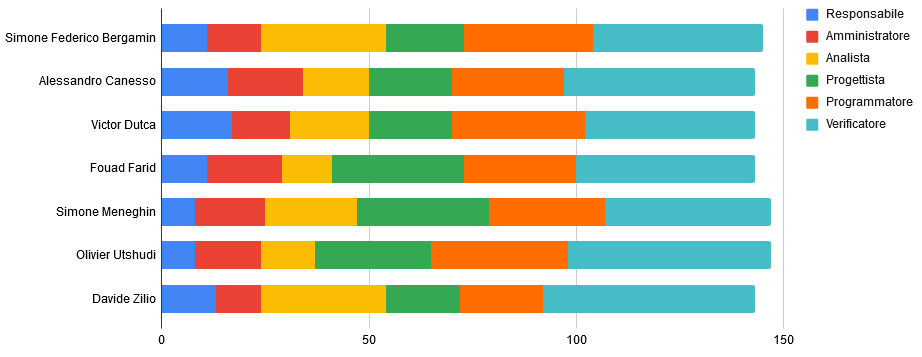
\includegraphics[scale=0.60]{img/grafici/tabella_tot_con_analisi.png}
\caption{Istogramma della ripartizione delle ore totali per ruolo con investimento}
\end{figure}

\paragraph{Prospetto economico} \mbox{} \\ \mbox{} \\
Il costo totale con investimento è riportato nella seguente tabella:

%tabella costi
\begin{table}[H]
\centering\renewcommand{\arraystretch}{1.5}
\caption{Costi totali con investimento}
\vspace{0.2cm}
\begin{tabular}{ c c c }
\rowcolor{redafk}
\textcolor{white}{\textbf{Ruolo}} & \textcolor{white}{\textbf{Ore}} & 
\textcolor{white}{\textbf{Costo}}  \\
Responsabile & 84 & 2520€ \\
Amministratore & 107 & 2140€ \\
Analista & 142 & 3550€ \\
Progettista	& 169 & 3718€ \\
Programmatore & 198 & 2970€  \\
Verificatore & 311 & 4665€  \\
\rowcolor{lastrowcolor}
\textbf{Totale} & \textbf{1011} & \textbf{19563€}  \\
\end{tabular}
\end{table}

I dati ottenuti si possono riassumere nel seguente areogramma:
\begin{figure}[H]
\centering
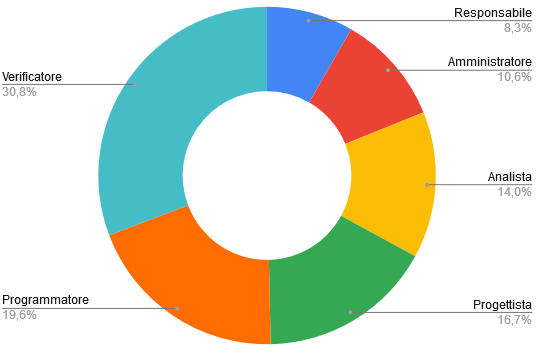
\includegraphics[scale=0.60]{img/grafici/torta_tot_con_analisi.png}
\caption{Areogramma della ripartizione dei costi totali per ruolo con investimento}
\end{figure}

\subsubsection{Ore rendicontate senza investimento}
\paragraph{Distribuzione oraria} \mbox{} \\ \mbox{} \\
Le ore rendicontate sono riassunte nella seguente tabella:

%tabella ore
\begin{table}[H]
\centering\renewcommand{\arraystretch}{1.5}
\caption{Distribuzione totale delle ore dell'intero progetto senza investimento}
\vspace{0.2cm}
\begin{tabular}{ c c c c c c c c }
\rowcolor{redafk}
\textcolor{white}{\textbf{Nominativo}} & \textcolor{white}{\textbf{Re}} & 
\textcolor{white}{\textbf{Am}} & \textcolor{white}{\textbf{An}} &
\textcolor{white}{\textbf{Pt}} & \textcolor{white}{\textbf{Pm}} &
\textcolor{white}{\textbf{Ve}} & \textcolor{white}{\textbf{Totale}} \\
Simone Federico Bergamin 	& 5 	& 6 	& 10	& 19	& 31	& 32 	& 103 \\
Alessandro Canesso 			& 8 	& 12	& - 	& 20	& 27	& 34 	& 101 \\
Victor Dutca 				& 8 	& 14	& 4 	& 20	& 32	& 25 	& 103 \\
Fouad Farid					& 4 	& 11	& - 	& 26	& 27	& 35 	& 103 \\
Simone Meneghin 			& 8 	& 9 	& 8 	& 22	& 28	& 30 	& 105 \\
Olivier Utshudi 			& 8 	& 8 	& - 	& 20	& 33	& 36 	& 105 \\
Davide Zilio 				& 9 	& 6 	& 13	& 18	& 20	& 37 	& 103 \\
\rowcolor{lastrowcolor}
\textbf{Ore totali ruolo} & \textbf{50} & \textbf{66} & \textbf{35} & \textbf{145} & \textbf{198} & \textbf{229} & \textbf{723} \\
\end{tabular}
\end{table}

Una rappresentazione visiva della suddivisione oraria viene data dal seguente grafico:
\begin{figure}[H]
\centering
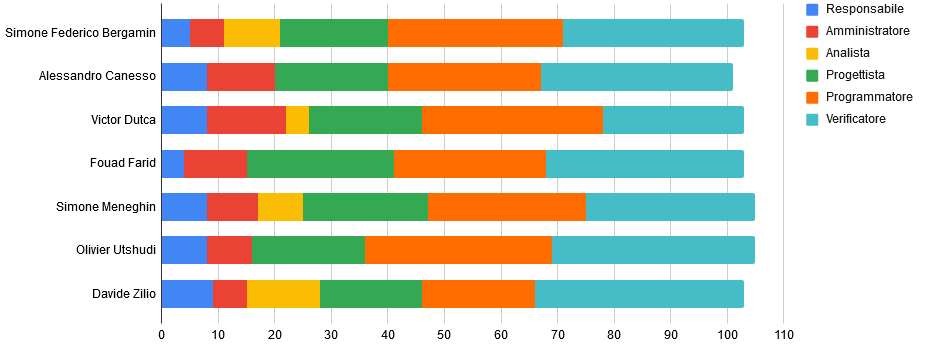
\includegraphics[scale=0.60]{img/grafici/tabella_tot_no_analisi.png}
\caption{Istogramma della ripartizione delle ore totali per ruolo con investimento}
\end{figure}

\paragraph{Prospetto economico} \mbox{} \\ \mbox{} \\
Il costo totale senza investimento è riportato nella seguente tabella:

%tabella costi
\begin{table}[H]
\centering\renewcommand{\arraystretch}{1.5}
\caption{Costi totali senza investimento}
\vspace{0.2cm}
\begin{tabular}{ c c c }
\rowcolor{redafk}
\textcolor{white}{\textbf{Ruolo}} & \textcolor{white}{\textbf{Ore}} & 
\textcolor{white}{\textbf{Costo}}  \\
Responsabile & 50 & 1500€ \\
Amministratore & 66 & 1320€ \\
Analista & 35 & 875€ \\
Progettista	& 145 & 3190€ \\
Programmatore & 198 & 2970€  \\
Verificatore & 229 & 3435€  \\
\rowcolor{lastrowcolor}
\textbf{Totale} & \textbf{723} & \textbf{13290€}  \\
\end{tabular}
\end{table}

I dati ottenuti si possono riassumere nel seguente areogramma:
\begin{figure}[H]
\centering
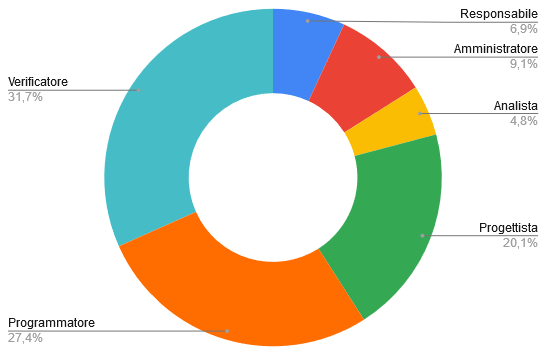
\includegraphics[scale=0.60]{img/grafici/torta_tot_no_analisi.png}
\caption{Areogramma della ripartizione dei costi totali per ruolo senza investimento}
\end{figure}

\subsection{Conclusioni}
Il costo totale preventivato per il progetto è 13.290,00€